\section{Results and Discussion}
\subsection{Length Calibration}

\begin{figure*}
	\centering
	\includegraphics[width=0.7\linewidth]{../plots/calibration.pdf}
	\caption{Silicon grid pattern for calibration.}
	\label{fig:calibration}
\end{figure*}

The initial task involved calibrating the instrument's length scale with a calibration grid.
\Cref{fig:calibration} displays the silicon grid pattern
used for calibration.
The orange dots indicate points used to assess the grid's periodicity.

Using the picture, the distances between adjacent points have
been calculated and averaged, whereby an average length of
$d_{\mathrm{sem}}=\qty{10.1 \pm 0.5}{\micro\meter}$ was determined.
The manufacturer of the silicon grid provides a periodicity length of
$d_{\mathrm{grid}}=\qty{9.87\pm 0.05}{\micro\meter}$.
This minor deviation can be corrected using a linear
correction function $d = \alpha d^*$, where $d$ is the calibrated
distance, $d^*$ the measured distance and
$\alpha=d_{\mathrm{grid}} /d_{\mathrm{sem}} = \num{0.977}$.
This calibration ensures that subsequent measurements are accurate.

\subsection{Investigation of an unknown semiconductor sample}
\paragraph{SED and BSE}
The next task of the lab course was to investigate an unknown sample
that exhibits artifically created structures, see \cref{fig:sample_0}.
The pictures were made in the vicinity of a crossing
point on which three vertical and three horizontal lines intersect.

With the help of different detector modes, it is possible to observe
different material properties.
The first picture, see \cref{subfig:sample_0_sed}, displays a recording
with an SED detector to obtain information about the sample's topography.
Surfaces of the same gray scale should have the same slope because of the
dependency $\delta_\mathrm{SE} \simeq \cos(\theta)$.
Horizontal and vertical grooves are visible, that were probably
fabricated by nanolithography.
At the intersections of the individual lines, additional structures can
be found.
Irregular chunks of crystallites can be seen, which indicate
some kind of crystal growth or residues from nanolithography.

The second and the third picture, see
\crefrange{subfig:sample_0_bsd_full}{subfig:sample_0_bsd_45}, display two
recordings captured with a BSD detector.
Both images have a lower resolution due to the larger area of
\ac{be}-interaction compared to \ac{se}-interaction.

\Cref{subfig:sample_0_bsd_full} illustrates an intensity
distribution where the signals from all BSD detectors have been combined.
The picture displays a clear intensity contrast between the large
homogeneous areas and the line bundles, therefore indicating a material
contrast.
The crystallites have a similar intensity as the large areas, so they
could originate from the same material.

\Cref{subfig:sample_0_bsd_45} presents a similar image, created by
combining signals from variously positioned detectors to simulate the
perspective of a detector positioned at the azimuthal angle of
\qty{45}{\degree} (at the top right of the image).
Differences are visible between the two BSD recordings: The right
half of the vertical lines and the upper half of the horizontal lines
are significantly darker than their opposite area.
Reason for this are no further material contrasts but rather the surface
topography and the position of the detector.
To be more precise, the side walls of the grooves are blocking the signal and
thus preventing the electrons	to reach the detector.

\paragraph{Distance calculation}
In \cref{subfig:sample_0_sed} there are also four distances labeled.
These distances are listed in \cref{tab:distances}.

\begin{table}[h]
	\centering
	\begin{tabular}{cccc}
		\toprule
		label & $d^*$ in \unit{\micro\meter} & $d$ in \unit{\micro\meter} \\
		\midrule
		1     & \num{3.0}                    & \num{2.93}                 \\
		2     & \num{4.76}                   & \num{4.65}                 \\
		3     & \num{3.04}                   & \num{2.97}                 \\
		4     & \num{2.59}                   & \num{2.53}                 \\
		\bottomrule
	\end{tabular}
	\caption{Characteristic distances of the sample.}
	\label{tab:distances}
\end{table}

\paragraph{EDX}
To get a better understanding of the sample's composition, one can
conduct an \ac{edx} spot analysis experiment.
In this lab course, three different spots, see \cref{subfig:edx_spots},
were chosen for two different electron energies:
\qty{10}{\kilo \electronvolt}
and \qty{20}{\kilo\electronvolt}.

The X-ray spectra for electrons with a kinetic energy of
\qty{10}{\kilo\electronvolt} for the selected spots are shown
in \crefrange{subfig:10kV_1_spectrum}{subfig:10kV_3_spectrum}.

The peak positions allow identification of the elements \ce{Ga},
\ce{As}, and \ce{Si}.
The corresponding elemental concentrations are evaluated with the help
of the data analysis program associated with the electron microscope and
are listed in \cref{tab:edx_1}.

The measurements of the first spot show that \ce{Ga} and \ce{As} are
the only constituents and are distributed in an equimolar ratio.
The measurement of the second spot returns \ce{Si} only.
The sample therefore consists of a silicon substrate with a
gallium arsenide thin film layer grown on top.
The material composition of the third spot is gallium arsenide,
with traces of silicon.

\begin{table}
	\centering
	\begin{tabular}{cccc}
		\toprule
		spot & element & $c_\mathrm{a}$ in \unit{\percent } & $c_\mathrm{m}$ in \unit{\percent} \\
		\midrule
		1    & Ga      & 50                                 & 49                                \\
		     & As      & 50                                 & 52                                \\
		\midrule
		2    & Si      & 100                                & 100                               \\
		\midrule
		3    & Ga      & 45                                 & 45                                \\
		     & As      & 49                                 & 53                                \\
		     & Si      & 6                                  & 3                                 \\
		\bottomrule
	\end{tabular}
	\caption{Atomic concentration percentage $c_\mathrm{a}$ and mass
		concentration percentage $c_\mathrm{m}$ measured at
		\qty{10}{\kilo\electronvolt}.}
	\label{tab:edx_1}
\end{table}

The X-ray spectra for electrons with a kinetic energy of
\qty{20}{\kilo \electronvolt} for the same spots are shown
in \crefrange{subfig:20kV_1_spectrum}{subfig:20kV_3_spectrum}.
The corresponding elemental concentrations are listed in
\cref{tab:edx_2}.
Small amounts of silicon are found at the first spot,
that was previously associated as a gallium arsenide thin film.
The reason for that is the penetration depth of the primary electrons,
which is a function of the kinetic energy.
Higher energies increase the penetration depth and therefore, primary
electrons can reach the first silicon layers.
This also explains the higher silicon concentration at the third spot.

\begin{table}
	\centering
	\begin{tabular}{cccc}
		\toprule
		spot & element & $c_\mathrm{a}$ in \unit{\percent } & $c_\mathrm{m}$ in \unit{\percent} \\
		\midrule
		1    & Ga      & 48                                 & 47                                \\
		     & As      & 48                                 & 51                                \\
		     & Si      & 4                                  & 2                                 \\
		\midrule
		2    & Si      & 100                                & 100                               \\
		\midrule
		3    & Ga      & 23                                 & 32                                \\
		     & As      & 26                                 & 39                                \\
		     & Si      & 51                                 & 29                                \\
		\bottomrule
	\end{tabular}
	\caption{Atomic concentration percentage $c_\mathrm{a}$ and mass
		concentration percentage $c_\mathrm{m}$ measured at
		\qty{20}{\kilo\electronvolt}.}
	\label{tab:edx_2}
\end{table}

In addition to spot analysis experiments, \ac{edx} maps can be used to
characterize large surface areas.
These maps display the varying atomic concentrations across the
surface, with each element represented by its own map.
As shown in \cref{fig:edx_maps}, the results support the
interpretation that the sample is a gallium arsenide thin film
on a silicon substrate.

\subsection{Layer thickness determination}
The last task was to determine the thickness of a notch that was
previously cut into the sample using an ion beam.
In order to do that, the sample was tilted by \qty{45}{\degree}.
The schematic representation of the notch geometry is shown
in \cref{fig:layer}.
With some trigonometric considerations and the distance
$d^*=\qty{1.04}{\micro\meter}$, that can be obtained from
\cref{fig:depth},
one finds the following formula for the layer thickness:
$t = d / \cos(\qty{45}{\degree}) = d^* \alpha / \cos(\qty{45}{\degree})
	= \qty{1.44}{\micro\meter}$.
\vfill

\begin{figure}[!h]
	\centering
	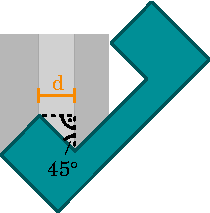
\includegraphics{../assets/angle.pdf}
	\caption{Geometrical arrangement of the tilted sample.}
	\label{fig:layer}
\end{figure}

\begin{figure*}[t!]
	\centering
	\begin{subfigure}{0.7\linewidth}
		\centering
		\includegraphics[width=\textwidth]{../plots/sample_1_SED.pdf}
		\caption{SED detector}
		\label{subfig:sample_0_sed}
	\end{subfigure}
	\begin{subfigure}{0.7\linewidth}
		\centering
		\includegraphics[width=\textwidth]{../plots/sample_1_BSD_full.pdf}
		\caption{BSD detector,  mode: BSD Full}
		\label{subfig:sample_0_bsd_full}
	\end{subfigure}
	\begin{subfigure}{0.7\linewidth}
		\centering
		\includegraphics[width=\textwidth]{../plots/sample_1_BSD_45.pdf}
		\caption{BSD detector, mode: BSD \qty{45}{\degree}}
		\label{subfig:sample_0_bsd_45}
	\end{subfigure}
	\caption{Various SEM images of the semiconductor sample.}
	\label{fig:sample_0}
\end{figure*}

\begin{figure*}
	\centering
	\begin{subfigure}{0.7\linewidth}
		\centering
		\includegraphics[width=\textwidth]{../plots/edx_10kV.pdf}
		\caption{spots used for \ac{edx} analysis}
		\label{subfig:edx_spots}
	\end{subfigure}
	\begin{subfigure}{0.45\linewidth}
		\centering
		\includegraphics[width=\textwidth]{../plots/edx_10kV_1_spectrum.pdf}
		\caption{\qty{10}{\kilo \electronvolt}, spot 1}
		\label{subfig:10kV_1_spectrum}
	\end{subfigure}
	\begin{subfigure}{0.45\linewidth}
		\centering
		\includegraphics[width=\textwidth]{../plots/edx_10kV_2_spectrum.pdf}
		\caption{\qty{10}{\kilo \electronvolt}, spot 2}
		\label{subfig:10kV_2_spectrum}
	\end{subfigure}
	\begin{subfigure}{0.45\linewidth}
		\centering
		\includegraphics[width=\textwidth]{../plots/edx_10kV_3_spectrum.pdf}
		\caption{\qty{10}{\kilo \electronvolt}, spot 3}
		\label{subfig:10kV_3_spectrum}
	\end{subfigure}
	\begin{subfigure}{0.45\linewidth}
		\centering
		\includegraphics[width=\textwidth]{../plots/edx_20kV_1_spectrum.pdf}
		\caption{\qty{20}{\kilo \electronvolt}, spot 1}
		\label{subfig:20kV_1_spectrum}
	\end{subfigure}
	\begin{subfigure}{0.45\linewidth}
		\centering
		\includegraphics[width=\textwidth]{../plots/edx_20kV_2_spectrum.pdf}
		\caption{\qty{20}{\kilo \electronvolt}, spot 2}
		\label{subfig:20kV_2_spectrum}
	\end{subfigure}
	\begin{subfigure}{0.45\linewidth}
		\centering
		\includegraphics[width=\textwidth]{../plots/edx_20kV_3_spectrum.pdf}
		\caption{\qty{20}{\kilo \electronvolt}, spot 3}
		\label{subfig:20kV_3_spectrum}
	\end{subfigure}
	\caption{X-ray spectra for different spots and electron energies.}
	\label{fig:edx_plots}
\end{figure*}

\begin{figure*}[t!]
	\centering
	\begin{subfigure}{0.45\linewidth}
		\centering
		\includegraphics[width=\textwidth]{../plots/map_As.pdf}
		\caption{\ce{As} }
		\label{subfig:map_as}
	\end{subfigure}
	\begin{subfigure}{0.45\linewidth}
		\centering
		\includegraphics[width=\textwidth]{../plots/map_Ga.pdf}
		\caption{\ce{Ga} }
		\label{subfig:map_ga}
	\end{subfigure}
	\begin{subfigure}{0.45\linewidth}
		\centering
		\includegraphics[width=\textwidth]{../plots/map_Si.pdf}
		\caption{\ce{Si} }
		\label{subfig:map_si}
	\end{subfigure}
	\caption{EDX concentration maps.}
	\label{fig:edx_maps}
\end{figure*}

\begin{figure*}[h]
	\centering
	\includegraphics[width=0.7\textwidth]{../plots/tilted.pdf}
	\caption{Image of the tilted sample .}
	\label{fig:depth}
\end{figure*}
